%-------------------------------------------------------------------
%	PACKAGES AND OTHER DOCUMENT CONFIGURATIONS
%-------------------------------------------------------------------

\documentclass[11pt,notitlepage]{article}

\usepackage{helvet} % Helvetica font

\usepackage[T1]{fontenc}

% Various AMS packages
\usepackage{amsfonts, amsmath, amsthm, amssymb} % For math fonts, symbols and environments

% More equation typesetting
\usepackage{commath}
\usepackage{physics}

\usepackage{graphicx} % Required for including images
\usepackage{caption}
\usepackage{booktabs} % Top and bottom rules for table

% Reduce the size of the margin
\usepackage[top=0.75in,bottom=0.75in,left=0.5in,right=0.5in]{geometry}

\usepackage{authblk}
\usepackage{hyperref}

% Typeset code
\usepackage{color}
\usepackage{xcolor}
\definecolor{lightlightgray}{gray}{0.9}

% For typesetting code
\usepackage{listings}
\lstset{
	numbers=left,  % line numbers
	numberstyle=\tiny,
	frame=tb,  % lines above and below the section
	xleftmargin=0.25in,
	xrightmargin=0.25in,
	tabsize=2,  % how many spaces are equivalent to \t
	breaklines=true,
	mathescape=true,  % allow inline math within listings environment
	backgroundcolor=\color{lightlightgray},  % (very) light gray background
	basicstyle=\ttfamily\footnotesize,
	%commentstyle=\color{cyan}\ttfamily,
	morecomment=[l][\color{blue}]{\#}
}

% Allow \texttt line wrapping
\usepackage[htt]{hyphenat}

% Header
\usepackage{fancyhdr}
\lhead{} % Remove subsection title from top-left of page
\renewcommand{\headrulewidth}{0pt}
\setlength{\headheight}{20pt} 

% Add a black line between paragraphs for readability
\usepackage[parfill]{parskip}

% More space between table entries
\renewcommand{\arraystretch}{1.2}

%\pagenumbering{gobble} % Removes page numbering
%\usepackage{mathrsfs}
%\usepackage{xfrac}
%\makeatother % Not sure what this does

\pagestyle{fancy}

%-------------------------------------------------------------------
%	MACROS
%-------------------------------------------------------------------

% Email
\newcommand{\email}[1]{\href{mailto:{#1}}{{#1}}}


% Italicized et al.
\newcommand{\etal}{\emph{et al.}}
\newcommand{\ie}{\emph{i.e.} }
\newcommand{\eg}{\emph{e.g.}}

% Operators
\newcommand{\dotprod}{\boldsymbol{\cdot}}
\newcommand{\kB}{k_{\text{B}}}

%%%%%%%%%
% LINKS %
%%%%%%%%%

% For the INDUS project
\newcommand{\repo}[1][GitHub]{\href{https://github.com/seanmarks/indus}{#1}}

% Home page for PLUMED
\newcommand{\PLUMED}{\href{http://www.plumed.org/}{PLUMED}}

% Google group for PLUMED users (have to add a \ before the #!)
\newcommand{\plumedusers}[1][link]{\href{https://groups.google.com/forum/\#!forum/plumed-users}{#1}}

% For PLUMED documentation
\newcommand{\plumedmanual}[1][link]{\href{https://plumed.github.io/doc.html}{#1}}

\newcommand{\plumeddoc}{https://plumed.github.io/doc-v2.4/user-doc/html}
\newcommand{\driver}{\href{\plumeddoc/driver.html}{\texttt{driver}}}
\newcommand{\installplumed}[1][link]{\href{\plumeddoc/_installation.html}{#1}}

% Home pages for MD engines
\newcommand{\GROMACS}{\href{http://www.gromacs.org/}{GROMACS}}
\newcommand{\LAMMPS}{\href{https://lammps.sandia.gov/}{LAMMPS}}
\newcommand{\AMBER}{\href{http://ambermd.org/}{AMBER}}
\newcommand{\NAMD}{\href{https://www.ks.uiuc.edu/Research/namd/}{NAMD}}

%-------------------------------------------------------------------
%	DOCUMENT
%-------------------------------------------------------------------

\begin{document}
	
% Prints the affiliations in a smaller, italicized font
\renewcommand\Affilfont{\itshape\small}
	
\title{INDUS\\User Manual}
\author{Sean M. Marks\\(\email{semarks@seas.upenn.edu})\\Amish J. Patel*\\(\email{amish.patel@seas.upenn.edu})}
\affil{Patel Group\\University of Pennsylvania}
	
% Uncomment this to hide the date
%\date{}

\maketitle
\tableofcontents

%%%

\section{Introduction}

The INDUS code described here computes the number of particles, $N_v$, and the coarse-grained number of particles, $\tilde{N}_v$, in probe volumes, $v$, of several different geometries. It is primarily intended to be used as an extension to \PLUMED, a popular plugin for molecular dynamics (MD) engines such as \GROMACS, \LAMMPS, \AMBER, and \NAMD. As part of PLUMED, the INDUS code can be used to post-process trajectories stored in a variety of formats (see \driver). If PLUMED+INDUS is subsequently patched into an MD engine, it can be used to perform biased simulations with $\tilde{N}_v$.

Note that INDUS can also be compiled as a standalone code. However, this is intended primarily for development purposes.

For more on the INDUS method in theory and practice, here is a (non-exhaustive) list of topics and relevant references:
\begin{itemize}
	\item INDUS for beginners \cite{Patel2010}
	\item INDUS in probe volumes of all shapes and sizes \cite{Patel2011}
	\item INDUS for biological systems, especially proteins \cite{Patel2012,Patel2014}
	\item INDUS and the sparse sampling method, an alternative to traditional umbrella sampling for efficiently computing $F_v(\tilde{N})$ \cite{Xi2016,Xi2018}
\end{itemize}

%%%

\subsection{Units}

The INDUS code uses the same basic set of units as PLUMED, which also happens to be the same as GROMACS.

% Units
\begin{center}
	\begin{tabular}{| c c |} 
		\hline
		\textbf{Quantity} & \textbf{Units} \\
		\hline
		Length & nm = $10^{-9}$ m = 10 \AA \\
		Time   & ps = $10^{-12}$ s \\
		Mass   & amu \\
		\hline
		Energy & kJ/mol \\
		\hline
	\end{tabular}
\end{center}

%%%

\section{Getting the Code}

The code is publicly available on GitHub (\repo[link]).

%%%

\section{Installation}

The following section details the ways in which INDUS can be installed.

%%%

\subsection{Patching INDUS into PLUMED}

It is recommended that you make use of the INDUS code as an extension to \PLUMED. Make sure that you perform the following steps \textbf{before} configuring and compiling PLUMED! 

A shell script to aid you in the patching process is available in the INDUS code repository under \texttt{indus/plumed\_patch/patch\_plumed.sh}. When you run the script, simply pass to it the location of the root directory of the PLUMED repository (\emph{i.e.} the one that contains the \texttt{Makefile} and so on):

\begin{lstlisting}
./patch_plumed.sh <location-of-PLUMED-source-code>
\end{lstlisting}

Then simply configure, compile, and install PLUMED normally. For instructions on how to install PLUMED, see \installplumed[here]. For those who are already using PLUMED, I recommend making a separate installation for PLUMED+INDUS.

Once installation is complete, a new action, \texttt{INDUS}, will be available to you the next time you run PLUMED. You can check that the procedure was successful by running the following command:

\begin{lstlisting}
plumed --no-mpi manual --vim --action INDUS
\end{lstlisting}

This will print out a list of all the actions and command-line tools registered in PLUMED, followed by options which are specific to the \texttt{INDUS} action. (\emph{Note}: The \texttt{--no-mpi} option flag is to prevent PLUMED from looking for an MPI library, since none is required for this check. The \texttt{--vim} flag causes output to be printed in a console-friendly format.)

%%%

\subsection{Patching PLUMED+INDUS into an MD Code}

Once you have installed PLUMED+INDUS, follow the instructions \href{\plumeddoc/_installation.html#Patching}{here} to add it to your MD engine of choice. Note that a given version of PLUMED only supports certain versions of each MD code. To check which MD codes and versions are supported by each version of PLUMED, check out the online manual (\plumedmanual).

%%%

\subsection{Installing INDUS as a Standalone Program}

The INDUS code can be compiled as a standalone program that can analyze XTC files. Before proceeding, you will need to install the \texttt{xdrfile} library written by the GROMACS development team (see \href{http://www.gromacs.org/Developer_Zone/Programming_Guide/XTC_Library}{here}). Make note of where you install it: you will need this information later.

Once you have installed \texttt{xdrfile}, go to the main directory of the INDUS code repository and change the following lines in the \texttt{Makefile}:

\begin{lstlisting}[mathescape=false]
# This variable indicates where you installed xdrfile (i.e. the directory containing 
# the folders bin, include, and lib).
XDR_DIR=$(HOME)/programs/xdrfile/1.1.4

# If you aren't using a compiler that supports MPI, change the following lines
# - Mac OSX: CC=clang, CXX=clang++
# - Linux: CC=gcc, CXX=g++
CC=mpicc
CXX=mpic++

# Change this variable to 0 (false) if you aren't using MPI compilers
is_mpi_enabled=1
\end{lstlisting}

%%%%%%

\section{Using the Code}


This section discusses how to use the INDUS code as part of PLUMED, and as a standalone code. Section \ref{sec:input} will discuss the details of the INDUS input file (\texttt{indus.input}). Note that this file is separate from the normal PLUMED input file (\texttt{plumed.dat}) and uses a different syntax. If you are not familiar with the input syntax for PLUMED, please consult the online manual for your version of choice (\plumedmanual).

%%%

\subsection{As Part of PLUMED}

Below is a sample PLUMED input file. Observe that the INDUS input file, \texttt{indus.input}, is an input to the \texttt{INDUS} action.

\begin{lstlisting}
# plumed.dat - PLUMED input file

# Create an instance of the INDUS action, which governs the interface between
# PLUMED and the INDUS code
indus: INDUS INPUTFILE=indus.input

# Put a harmonic bias on Ntilde_v of the form U = KAPPA/2*(Ntilde_v - AT)^2,
# where KAPPA=0.5 kJ/mol and AT=3
restraint: RESTRAINT ARG=indus.ntilde KAPPA=0.5 AT=3.0

# Print some important quantities
# - indus.n        = N_v
# - indus.ntilde   = Ntilde_v
# - restraint.bias = value of the biasing potential
# - STRIDE=500     = print every 500 steps (i.e. every 1 ps when dt=0.002ps)
PRINT ...
	LABEL=print
	ARG=indus.n,indus.ntilde,restraint.bias
	STRIDE=500
	FILE=plumed.out
... PRINT
\end{lstlisting}

%%%

\subsection{As a Standalone Program (XTC files only)}

When compiled as a standalone program, the INDUS code can be used to analyze XTC files. Invoke from the command line using the following syntax:

\begin{lstlisting}
./indus <indus.input>
\end{lstlisting}

See Section \ref{sec:input_standalone} for input options particular to running in standalone mode.

%%%%%%

\subsection{Limitations of the Code and Warnings to Users}

\begin{enumerate}
	\item Only orthorhombic boxes are supported (i.e. rectangular box where the side lengths may differ from each other)
	
	\item Periodic boundary conditions (PBCs) in all directions are assumed.
	
	\item Unless specified otherwise, probe volumes should not cross the periodic boundaries.
	
	\item Only one probe volume may be specified per instance of INDUS.
	
	\item The only indicator/switching functions supported for INDUS are the ones outlined in refs. \cite{Patel2010,Patel2011}. Unlike most of PLUMED's switching functions, these have continuous first derivatives and therefore produce smooth forces.
	
	\item You should be able to pass \texttt{indus.ntilde} and \texttt{indus.ubias} to any other PLUMED action with no problems. For example, it should be possible to perform metadynamics with $\tilde{N}_v$. However, I have not tested this aside from passing \texttt{indus.ntilde} and \texttt{indus.ubias} to \texttt{RESTRAINT}.
	
	\item I used PLUMED 2.4.0 and GROMACS 2016.3 when writing and testing the code. Any other versions of PLUMED that are 2.2 or higher should work just fine, but I have not tested these and cannot guarantee that they will work. The program should run fine with any simulation package that your favorite PLUMED version supports, but---again---I haven't tested it myself.
\end{enumerate}

% INPUT OPTIONS

\section{Input Options}{\label{sec:input}}

This section discusses the syntax of the INDUS input file, which is typically named \texttt{indus.input}. For more on the input syntax for PLUMED, consult the online manual (\plumedmanual).

\emph{Note:} In the following section, angle brackets (\texttt{<>}) are used to indicate places where a value should be placed. The angle brackets themselves are not part of the actual input syntax. Vertical lines (\texttt{|}) are used to enumerate options when only a limited number of values are permitted. For example, \texttt{axis = <x|y|z>} indicates that you must choose \texttt{axis} to be either \texttt{x}, \texttt{y}, or \texttt{z}.

%%%%%%

\subsection{Input File Structure}

The INDUS input file is organized into key-item pairs, where the \emph{item} can be one of the following: 
\begin{enumerate}
	\item a \emph{value}: a string or number
	\item a \emph{vector}: a sequence of values enclosed by square brackets, [ \ ]. Sometimes I will also use the term \emph{array}, which is simply a vector that has a fixed number of values.
	\item a \emph{block}: an arbitrary grouping of values, vectors, and possibly other blocks, all enclosed by curly braces, { \ }. A block functions like an object (in the sense of object-oriented programming) and all of the entries within its curly braces are said to be in its \emph{scope}.
\end{enumerate}

It is instructive to consider an example:

\begin{lstlisting}
MyBlock = {
	# This is a comment
	some_value  = 2.718
	some_vector = [ 1.0  2.0  3.0 ]   # This is a comment at the end of a line
	
	# Presumably, MyBlock corresponds to an object in the code that owns 
	# another object of type NestedBlock
	NestedBlock = {
		another_value = 3.14159
		AnotherBlock = { another_vector = [ we are values ] }
	}
}
\end{lstlisting}

Observe that each key is separated from its corresponding item by an equals sign (\texttt{=}). Comments are indicated by the hash character (\texttt{\#}). Each token in the input file (e.g. keys, values, equals signs, brackets, braces, comment characters, etc.) must be separated from the others by whitespace (single/multiple spaces or a new line). 

Aside from the aforementioned restrictions, the input syntax is quite flexible. Indentation is not necessary, and braces/brackets/equals signs need not be on the same line as any other token. For example, the following is an eyesore but perfectly legal:

\begin{lstlisting}
MyBlock 
= { some_vector = [ 
1.0  2.0  
3.0 ] }
\end{lstlisting}

%%%

Each key-item pair exists within a scope. The highest scope in the input file is the \emph{file scope}. This encompasses all the values, vectors, and blocks that are not enclosed in other blocks. For instance, \texttt{MyBlock} in the previous examples is a block at file scope. In contrast, \texttt{NestedBlock} and \texttt{some\_vector} are within the scope of \texttt{MyBlock}. In this way of thinking, the input file \emph{itself} is like an object at the top of the hierarchy.

%%%%%%

\subsection{Target Atom Selection}

Target atoms are indicated by the key \texttt{Target} at file scope. This is a unique key, \emph{i.e.} multiple target selections are not permitted.

\subsubsection{By Index}

Atoms are selected as ranges of indices of the form \texttt{<start>-<stop>:<stride>}, the same as in PLUMED. This selects every \texttt{<stride>}th atom from index \texttt{start} to \texttt{stop}. All indices start at 1. if \texttt{:<stride>} is omitted, the stride is assumed to be 1.

Here are some examples.

\begin{lstlisting}
# Select every 4th atom from index 1 to index 16500
Target = [ atom_index 1-16500:4 ]

# Select every atom from index 500 to index 1000
Target = [ atom_index 500-1000 ]

# Ranges can be combined using a comma (no spaces)
Target = [ atom_index  1-16500:4,32000-64000:3 ]
\end{lstlisting}

%%%

\subsection{Probe Volume Geometries}

Probe volumes are defined at global scope using the keyword \texttt{ProbeVolume}. Only one probe volume geometry may be specified per instance of INDUS. To define multiple probe volumes using PLUMED, one must create multiple instances of the \texttt{INDUS} action.

Each probe volume definition includes two coarse-graining parameters: $\sigma$
(\texttt{sigma}) and $\alpha_c$ (\texttt{alpha\_c}). These determine how closely the coarse-grained number of particles, $\tilde{N}$, is correlated with the integer number of particles, $N$. For a detailed explanation, see refs. \cite{Patel2010} and \cite{Patel2012}. In short, choosing smaller values leads to tighter correlation between $\tilde{N}$ and $N$, but larger forces. This can cause instability and simulation crashes if $\sigma$ and/or $\alpha_c$ are chosen too small. 

We recommend the values $\sigma = 0.01$ nm and $\alpha_c = 2 \sigma = 0.02$ nm for simulations of water; these are the defaults if \texttt{sigma} and \texttt{alpha\_c} are omitted from the \texttt{ProbeVolume} definition. In practice, we have found that these values lead to stable simulations with tight correlation between $N$ and $\tilde{N}$, to the extent that we consider the two essentially interchangeable.

The following subsections describe the syntax for the probe volume geometries currently supported.

%%%

\subsubsection{Sphere}

\begin{lstlisting}
ProbeVolume = {
  type   = sphere
  r_max  = <$r$>
  center = [ <$x$>  <$y$>  <$z$>  ]
  # Coarse-graining
  sigma   = <$\sigma$>
  alpha_c = <$\alpha_c$>
}
\end{lstlisting}

%%%%%%

\subsubsection{Box}

\begin{lstlisting}
ProbeVolume = {
	type   = box
	# Boundaries of box along each axis
	x_range = [ <$x_{\text{min}}$> <$x_{\text{max}}$> ]
	y_range = [ <$y_{\text{min}}$> <$y_{\text{max}}$> ]
	z_range = [ <$z_{\text{min}}$> <$z_{\text{max}}$> ]
	# Coarse-graining
	sigma   = <$\sigma$>
	alpha_c = <$\alpha_c$>
}
\end{lstlisting}

%%%%%%

\subsubsection{Cylinder}

\begin{lstlisting}
ProbeVolume = {
	type   = cylinder
	# Cylinder will have its axis parallel to this axis 
	# - Default: parallel to $z$-axis
	axis    = <x|y|z>
	# Location of the center of the base
	base    = [ <$x$>  <$y$>  <$z$>  ]
	radius  = <$r$>
	height  = <$h$>
	# Coarse-graining
	sigma   = <$\sigma$>
	alpha_c = <$\alpha_c$>
}
\end{lstlisting}

%%%%%%

\subsection{Biasing $\tilde{N}_v$ Using the INDUS Code's Potential}

Recall that PLUMED's \texttt{RESTRAINT} action can be used to set the form of the biasing potential on $\tilde{N}_v$. As an alternative, the INDUS code makes available makes available its own biasing potential of the following general form:

\begin{align}
	\mathcal{U}_{\text{bias}}(x) 
	&= \mathcal{U}_{\text{harmonic}}(x) + \mathcal{U}_{\text{linear}}(x)
	     + \mathcal{U}_{\text{left harmonic}}(x) + \mathcal{U}_{\text{right harmonic}}(x) \\
	\label{eqn:generalbias}
	&= \frac{1}{2} \kappa (x - x^*)^2 + (\phi x + c)
	   + \frac{1}{2} k_{\text{left}}  (x - x_{\text{left}})^2 \Theta(x_{\text{left}} - x)
	   + \frac{1}{2} k_{\text{right}} (x - x_{\text{right}})^2 \Theta(x - x_{\text{right}})
\end{align}

\noindent where $\Theta(x)$ is the unit step function, which is zero for $x < 0$ and one for $x \ge 1$. Note that PLUMED supports similar functionality with a combination of the \texttt{RESTRAINT}, \texttt{LOWERWALLS}, and \texttt{UPPERWALLS} actions.

The corresponding syntax for the INDUS input file is:

\begin{lstlisting}
Bias = {
	# Tells INDUS that x=Ntilde_v
	order_parameter = ntilde

	# Harmonic
	x_star = <$x^*$>
	kappa  = <$\kappa$>

	# Linear
	phi      = <$\phi$>
	constant = <$c$>

	# Left one-sided harmonic
	x_left = <$x_{\text{left}}$>
	k_left = <$k_{\text{left}}$>

	# Right one-sided harmonic
	x_right = <$x_{\text{right}}$>
	k_right = <$k_{\text{right}}$>
}
\end{lstlisting}

\noindent Any parameters not specified in the input file are set to zero automatically.

%%%

Then, in the PLUMED input file, \texttt{RESTRAINT} is called with \texttt{ARG}$ = \mathcal{U}_{\text{bias}}(\tilde{N}_v)$. This is done to ensure that the biasing forces are correctly passed to the PLUMED core.

\begin{lstlisting}
restraint: RESTRAINT ARG=indus.ubias SLOPE=1.0 AT=0.0 KAPPA=0.0
\end{lstlisting}

%%%%%%

\subsection{Standalone Mode Options}{\label{sec:input_standalone}}

The following options are supported at file scope.

\begin{lstlisting}
# The XTC file to analyze
XtcFile = <path_to_file>

# Range of times for which calculations are performed (in ps)
t0 = <$t_0$>
tf = <$t_f$>
\end{lstlisting}

\noindent All of these options are ignored when running the INDUS code as part of PLUMED.

%%%%%%

\section{Examples}

%%%

\subsection{Post-Processing a Trajectory with PLUMED's \texttt{driver}}

Suppose that we have run simulation (biased or unbiased) and would now like to compute $N$ and $\tilde{N}_v$ for each frame of the trajectory, which is saved as an XTC file named \texttt{traj\_comp.xtc}. The probe volume is a cylinder with the center of its base at $\mathbf{r}_0 = (2.0, 2.0, 2.0)$ nm with radius $r = 1.0$ nm and height $h = 0.5$ nm. The cylinder is parallel to the $y$-axis and extends from $y_{\text{low}} = 2.0$ nm to $y_{\text{high}} = y_{\text{low}} + h = 2.5$ nm. The target atoms have indices 1, 4, 7, ... , 16498 (i.e. every 3 atoms from 1 to 16,500, indexed from 1). The coarse-graining parameters are $\sigma = 0.01$ nm and $\alpha_c = 2 \sigma = 0.02$ nm.

The INDUS input file will be:
\begin{lstlisting}
# indus.input

# Atoms targeted by INDUS
Target = [ atom_index 1-16500:3 ]

# Probe volume
ProbeVolume = {
	type   = cylinder
	axis   = y
	# Dimensions and location
	base   = [ 2.0 2.0 2.0 ]
	r_max  = 1.0
	height = 0.5
	# Coarse-graining
	sigma   = 0.01
	alpha_c = 0.02
}
\end{lstlisting}

\noindent The corresponding PLUMED input file is:
\begin{lstlisting}
# plumed.dat

# Create an instance of the INDUS action, which computes N_v and Ntilde_v
indus: INDUS INPUTFILE=indus.input

# Print N_v and Ntilde_v for each frame to a file named 'plumed.out'
PRINT ...
	LABEL=print
	ARG=indus.n,indus.ntilde
	FILE=plumed.out
... PRINT
\end{lstlisting}

%%%

PLUMED's \texttt{driver} can be invoked from the command line as follows:

\begin{lstlisting}
plumed driver --plumed "plumed.dat" --ixtc "traj_comp.xtc"
\end{lstlisting}

For more \texttt{driver} options---including how to post-process trajectories in other file formats---please consult the PLUMED manual.

%%%

\subsection{Running a Biased Simulation with PLUMED}

Suppose we want to run a biased simulation with a linear umbrella sampling potential on $\tilde{N}_v$. The probe volume and target atoms are the same as in the last example. Use PLUMED's \texttt{RESTRAINT} action to apply a bias of the form $\mathcal{U}_{\text{bias}} = \phi \tilde{N}$ with $\phi = 0.6$ kJ/mol.

The INDUS input file is unchanged from before. The PLUMED input now contains an instance of \texttt{RESTRAINT}, as follows:
\begin{lstlisting}
# plumed.dat

# Create an instance of the INDUS action, which computes N_v and Ntilde_v
indus: INDUS INPUTFILE=indus.input

# Put a linear bias on Ntilde_v
restraint: RESTRAINT ARG=indus.ntilde SLOPE=0.6 AT=0.0

# Print N_v, Ntilde_v, and U_bias every 500 steps
PRINT ...
	LABEL=print
	ARG=indus.n,indus.ntilde,restraint.bias
	STRIDE=500
	FILE=plumed.out
... PRINT
\end{lstlisting}

%%%

The syntax for passing this PLUMED input file to the MD engine will depend on your choice of MD engine. Please consult the PLUMED manual for details (\plumedmanual).

%%%

\subsection{Standalone Mode}

Post-process a trajectory stored as an XTC file named \texttt{my\_trajectory.xtc}. Compute $N_v$ and $\tilde{N}_v$ in a spherical probe volume centered at $\mathbf{r}_0 = (2.5, 2.5, 2.5)$ nm and with radius $r = 0.6$ nm. The target atoms have indices 1, 5, 9, ... , 16497 (i.e. every 4 atoms from 1 to 16,500, indexed from 1). The coarse-graining parameters are $\sigma = 0.01$ nm and $\alpha_c = 2 \sigma = 0.02$ nm. Print the time series of $N_v$ and $\tilde{N}_v$ for $t \ge 100$ ps and $t \le 500$ ps. Also print the forces that would be obtained for these frames under a harmonic potential on $\tilde{N}_v$ with $\kappa = 0.98$ kJ/mol and $N^* = -5$.

\begin{lstlisting}
# indus.input

# Atoms targeted by INDUS
Target = [ atom_index 1-16500:4 ]

# Probe volume
ProbeVolume = {
	type   = sphere
	center = [ 2.5 2.5 2.5 ]
	r_max  = 0.6
	# Coarse-graining
	sigma   = 0.01
	alpha_c = 0.02
}

# Add a harmonic bias
Bias = {
	order_parameter = ntilde
	x_star = -5
	kappa  = 0.98
}

# XTC file to analyze
XtcFile = my_trajectory.xtc

# Production phase (ps)
t0 = 100
tf = 500

# Print time series of N_v and Ntilde_v, and biasing forces
PrintOutput = yes
PrintForces = yes
\end{lstlisting}

% BIASING PARAMETERS

\section{Choice of Biasing Parameters for Umbrella Sampling}

When performing umbrella sampling with $\tilde{N}_v$ to obtain the free energy landscape, $F_v(\tilde{N}) = -\kB T \ln P_v(\tilde{N})$, the parameters in the biasing potential used must be chosen carefully to ensure accurate results. Appropriate heuristics for choosing the parameters will depend upon the system of interest, the form of the potential(s) used, and the features of its expected free energy landscape. Here, I will present heuristics that we have found useful for biasing $\tilde{N}_v$ in atomistic simulations of dense liquids.

%%%

Suppose that we want to bias $\tilde{N}_v$ using a harmonic potential,

\begin{equation} \label{eqn:harmonicbias}
	\mathcal{U}_{\text{bias}}(\tilde{N}_v) = \frac{1}{2} \kappa (\tilde{N}_v - N^*)^2,
\end{equation}

\noindent where $\kappa$ and $N^*$ are constants (the biasing parameters). For INDUS in dense liquids such as water, we use the statistics of $N_v$ in the liquid basin in an unbiased simulation to guide our choice of biasing parameters. Let the average and variance of $N_v$ in the liquid basin be $\langle N_v \rangle_0$ and $\langle (\delta N_v)^2 \rangle_0$, respectively. Assuming that the liquid basin is approximately Gaussian, its curvature is

\begin{equation}
	\kappa_0 = \frac{k_{\text{B}} T}{\langle (\delta N_v)^2 \rangle_0}
\end{equation}

%%%

For most systems of interest, we have found that $\kappa_0$ is a decent estimate of the maximum curvature of the underlying landscape, $F_v(\tilde{N})$. We therefore choose $\kappa$ as a multiple of $\kappa_0$:

\begin{equation}
	\kappa = \alpha \kappa_0
\end{equation}

\noindent where $\alpha = 2$ or $3$. 

%%%

Accurate WHAM results also require overlap of the biased free energy landscapes, $F_v^{(\kappa, N^*)}(\tilde{N})$, between adjacent windows. For a desired overlap of $ \Delta F_{\text{overlap}}$, assuming that the biased ensembles for each $N^*$-value are Gaussian leads an estimated spacing between $N^*$-values of

\begin{equation}
	\Delta N^* = 2 \sqrt{ \frac{(\beta \Delta F_{\text{overlap}}) \langle (\delta N_v)^2 \rangle_0}{1 + \alpha} }
\end{equation}

%%%

\noindent where $\beta = (\kB T)^{-1}$. For an initial guess, we typically choose $\alpha = 2$ and $\Delta F_{\text{overlap}} = 4 \ k_{\text{B}} T$. This leads to:

\begin{align}
	\label{eqn:kapparule}
	\kappa &= 2 \kappa_0  \\
	\label{eqn:nstarrule}
	\Delta N^* &= \frac{4}{\sqrt{3}} \sqrt{ \langle (\delta N_v)^2 \rangle_0 }
\end{align}


Note that sampling $N_v = 0$ may require you to use windows with $N^* < 0$.

%%%

\subsection{Example: Umbrella Sampling in Bulk Water}

To illustrate the heuristics outlined above, I describe here the procedure to compute the free energy as a function of $\tilde{N}$, $F_v(\tilde{N})$, in a sphere (radius $r = 0.6$ nm) in bulk water at 300 K and 1 bar. Since it is infeasible to use standard MD simulations to sample $\tilde{N}$ outside of a narrow range near $\langle N \rangle_0$, an enhanced sampling technique is required. I chose to use umbrella sampling \cite{Torrie1977,Patel2010}. Sample \lstinline|plumed.dat| and \lstinline|indus.input| input files are available in the code repository under \lstinline|manual/examples/bulk_water|.

All simulations were performed using GROMACS 2016.3 \cite{VanDerSpoel2005}, patched with an installation of PLUMED+INDUS based on PLUMED 2.4.0 \cite{Tribello2014}. The simulation consisted of about 4,000 SPC/E water molecules \cite{Berendsen1987} in a square box. The temperature was maintained at $T = 300$ K using the stochastic velocity rescale thermostat \cite{Bussi2007} with a time constant of $\tau_T = 0.5$ ps, and the pressure was maintained at $P = 1$ bar using an isotropic Parrinello-Rahman barostat \cite{Parrinello1981} with time constant $\tau_P = 2$ ps. The simulation was run for 2 ns with the leapfrog integrator and a time step of 2 fs. Samples were taken every 1 ps (500 steps).

First, I performed an unbiased simulation to guide the choice of biasing parameters for a harmonic potential (see Equation \ref{eqn:harmonicbias}). I discarded the first 500 ps and used the remaining frames to compute $\langle N_v \rangle_0 \approx 30$ and $\langle (\delta N_v)^2 \rangle_0 \approx 5.09855$. From this, I computed $\kappa \approx 0.98$ kJ/mol and $\Delta N^* \approx 5$ using Equations \ref{eqn:kapparule} and \ref{eqn:nstarrule}. 

Using these parameters, I ran a series of biased simulations with $N^* = 25, 20, 15, 10, 5, 0, \text{ and } -5$ for 2 ns each. The INDUS coarse-graining parameters were $\sigma = 0.01$ nm and $\alpha_c = 2 \sigma = 0.02$ nm. I discarded the first 200 ps of each trajectory and used the remaining data (along with the data from the unbiased simulation) to compute the unbiased free energy distribution, $F_v( \tilde{N} )$, using UWHAM \cite{Tan2012}. Figure \ref{fig:fvn_bulk} illustrates the results. Note that if the free energy as a function of $N$ is desired, these results can be reweighted to obtain $F_v(N)$ (see ref. \cite{Patel2010}).

%%%

\begin{figure}
	\label{fig:fvn_bulk}
	\centering
	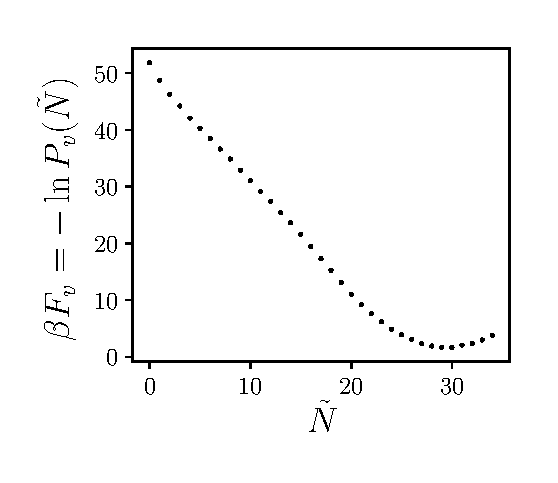
\includegraphics[width=0.5\textwidth]{examples/bulk_water/plot_F_v_Ntilde_WHAM.eps}
	\captionsetup{width=0.8\linewidth}
	\caption{\label{fig:fvn_bulk}The free energy landscape for the coarse-grained number of waters, $\tilde{N}$, in a small probe volume in bulk water at $T = 300$ K and $P = 1$ bar. The probe volume, $v$, is a sphere of radius $r = 0.6$ nm in a box of about $4,000$ SPC/E water molecules.}
\end{figure}

%%%

% DEVELOPMER NOTES

\section{Developer Notes}

This section is intended for those who wish to implement new probe volume geometries and/or understand the inner workings of the INDUS code. A working understanding of C++ is assumed. 

\textbf{NOTE:} This section currently under construction.

%%%

\subsection{Adding New Probe Volumes}

Implementing a new probe volume geometry is relatively simple. All geometries must be derived classes of abstract base class \texttt{ProbeVolume}, which handles the interface between particular geometries and the rest of the code. New probe volumes must implement the following methods:

\begin{itemize}
	\item Constructor
	\item \texttt{isInProbeVolume}: given the position of a particle $i$, this function returns a \texttt{bool} indicating whether or not the particle is in the nominal probe volume, \emph{i.e.} whether it contributes to $N_v$. It also computes indicator functions $h_v(i)$ and $\tilde{h}_v(i)$, the derivatives $\partial \tilde{h}_v(i) / \partial \mathbf{r}_i$, and whether the particle is in shell 1 or shell 2.
	\item (some other helper methods ...)
\end{itemize}

Additionally, you must register your probe volume with the INDUS driver. Each probe volume has a unique name associated with it, which I refer to as its \emph{type}. This corresponds to the \texttt{type} field when declaring a \texttt{ProbeVolume} in \texttt{indus.input}. For an example of how to do this, see the code at the top of \texttt{ProbeVolume\_Sphere.cpp}.

%%%

\subsubsection{What are the "shells"?}

As you look through the source code, you will see many references to "shell 1" and "shell 2." In the context of the probe volume, these are regions of space that are within a certain distance of the edges of the coarse-grained probe volume. You can think of shell 1 as the first coordination shell around the probe volume, and shell 2 as the second coordination shell. This functionality is not currently used, but will be important for future additions that I would like to make.

%%%

To make things more concrete, let $w_1$ and $w_2$ be the widths of shell 1 and shell 2, respectively. Consider a spherical probe volume with radius $r$ centered at point $\mathbf{r}_0$ that has coarse-graining parameters $\sigma$ and $\alpha_c$. A particle $i$ is assigned to different regions depending on its distance from the center of the sphere, $r_{i,0}$. Then

\begin{equation}
	\text{particle $i$ is in}
	\begin{cases}
		\text{the "nominal" probe volume, $v$,}
			& \text{for } r_{i,0} \leq r \\
		\text{the "coarse-grained" probe volume, $\tilde{v}$,}
			& \text{for } r_{i,0} \leq \tilde{r} \\
		\text{shell 1,}
			& \text{for } \tilde{r} < r_{i,0} \leq r_1 \\
		\text{shell 2,}
			& \text{for } r_1 < r_{i,0} \leq r_2
	\end{cases}
\end{equation}

\noindent where

\begin{align}
	\tilde{r} &= r + \alpha_c                       & \text{(outer radius of $\tilde{v}$)} \\
	r_1       &= \tilde{r} + w_1                    & \text{(outer radius of shell 1)} \\
	r_2       &= r_1 + w_2 = \tilde{r} + w_1 + w_2  & \text{(outer radius of shell 2)}
\end{align}

%%%

As mentioned previously, the shells are not currently used in the code but will be used in future versions to support new features. If you only care about doing standard INDUS, then you can just return \texttt{is\_in\_shell\_1 = false} and \texttt{is\_in\_shell\_2 = false} wherever applicable and the code will work just fine for INDUS.

%%%

\subsection{Parallelization with MPI}

% TODO
INDUS makes use of MPI to support limited parallelization within the PLUMED framework.

%%%




% REFERENCES

\bibliographystyle{unsrt}
\bibliography{references}

\end{document}